\documentclass[a4paper, 11pt]{article}

\usepackage[all]{xy}
\usepackage{fullpage}
\usepackage{graphicx}
\usepackage{amsmath}
\usepackage{amssymb}
\usepackage{amsthm}
\usepackage{amsthm}
\usepackage{fancyvrb}
\usepackage{tikz}
\usepackage{graphicx}
\usepackage{mathtools}
\usepackage{ tipa }
\usepackage[spanish]{babel}
\usepackage{verbatim}

\usepackage{tikz}

\usepackage[utf8]{inputenc} 

\usetikzlibrary{shapes,positioning,calc}
\colorlet{lightgray}{gray!20}

\usetikzlibrary{automata, arrows.meta, positioning}
\usetikzlibrary{quotes,angles}

\graphicspath{ {} }

\DeclareMathOperator{\arctg}{arctg}
\DeclareMathOperator{\car}{car}
\DeclareMathOperator{\ord}{ord}
\DeclareMathOperator{\mcd}{mcd}
\DeclareMathOperator{\mcm}{mcm}

\author{Javier Martínez Pérez, \\Sofía Maceín Sanz \\Nuria Jiménez Carrasco}
\title{Arthur Christmas, Bases de Datos}

\begin{document}

\maketitle

\theoremstyle{definition}
\newtheorem*{proy}{Arthur Christmas}
\newtheorem*{hipad}{Hipótesis adicionales}
\newtheorem*{noinc}{Requisitos no incluidos en el esquema}


%Changing the name of the most used math objects
\newcommand{\C}{\mathbb{C}}
\newcommand{\R}{\mathbb{R}}
\newcommand{\Q}{\mathbb{Q}}
\newcommand{\Z}{\mathbb{Z}}
\newcommand{\N}{\mathbb{N}}
\newcommand{\F}{\mathbb{F}}
\newcommand{\pmin}{m_{\alpha, K}}

\newcommand\restr[2]{{
  \left.\kern-\nulldelimiterspace 
  #1 % the function
  \vphantom{\big|} 
  \right|_{#2} 
  }}

\begin{proy}
	Santa Claus va a jubilarse y ya no realiza el reparto de los regalos de Navidad con su trineo volador. Su
	hijo mayor Steve ha modernizado el proceso, reemplazando el tradicional trineo por una enorme nave
	espacial, llamada S-1, que transporta un ejército de elfos de élite. Ellos son los encargados de realizar la
	tarea de Santa Claus, esto es, de repartir en una sola noche los regalos de los 600 millones de niños del
	planeta. La operación es controlada milimétricamente por los técnicos del centro de control del Polo
	Norte, que toman como referencia la información guardada en una base de datos ideada por Steve. Sin
	embargo, el hijo menor de Santa Claus, Arthur Christmas, no está conforme con el diseño del esquema
	y ha decidido realizar algunos cambios. Los requisitos que debe considerar son los siguientes:
	\begin{enumerate}
		\item Todo el personal involucrado en la Operación Regalo se distribuye en departamentos (código
		y nombre). Cada elfo (nombre, apellido y número de la seguridad social) pertenece a un
		único departamento y está contratado a tiempo completo o a tiempo parcial, ya que algunos
		de ellos también colaboran en la Operación Regalo de los Reyes Magos.
		\item Los elfos que son contratados a tiempo parcial realizan varias tareas específcas como la recogida
		de cartas y el empaquetado de los juguetes. Sin embargo, los contratados a tiempo completo son
		los únicos que pueden dirigir un departamento. Más exactamente, cada departamento es dirigido
		por uno de sus empleados a tiempo completo, el cual no puede participar en la dirección de ningún
		otro departamento.
		\item Los protagonistas de la Operación Regalo son los niños. De cada niño se guarda cuidadosamente
		el nombre y primer apellido, la fecha de nacimiento y las coordenadas de localización. Con
		el propósito de hacer un reparto justo de los regalos, cada niño es observado por un elfo que lo
		sigue en exclusiva durante todo el año. Se incluye la información de su(s) mascota(s) (si tiene)
		que consiste en el nombre, la especie y la edad. Cada mascota se registra una sola vez aunque
		esté al cuidado de varias personas, ya que lo que se pretende es evitar los problemas que pudiera
		causar durante la entrega de regalos.
		\item Para optimizar el reparto de regalos, se almacena información acerca de la relación de parentesco
		entre hermanos y hermanastros. Por ejemplo, Zipi y Zape son hermanos, hijos de Don Pantuflo
		Zapatilla y Doña Jaimita Llobregat. Sin embargo, Phineas y Candance son hijos de Linda Flynn
		e hijastros de Lawrence Fletcher, mientras que Ferb es hijo de Lawrence e hijastro de Linda.
		\item Tras la recogida de cartas, los elfos registran en la base de datos las peticiones de los niños. Para
		ello disponen de un gigantesco catálogo con las características de todos los juguetes disponibles:
		nombre, descripción, edad mínima recomendada, edad máxima recomendada y duración
		estimada. Durante el reparto de estos regalos, los elfos almacenan concienzudamente las entregas
		que se van realizando, asegurándose de que lo recibido por cada niño es lo que pidió en su carta.
	\end{enumerate}
\end{proy}


\begin{figure}
\part*{Esquema E/R}	
	\centering
	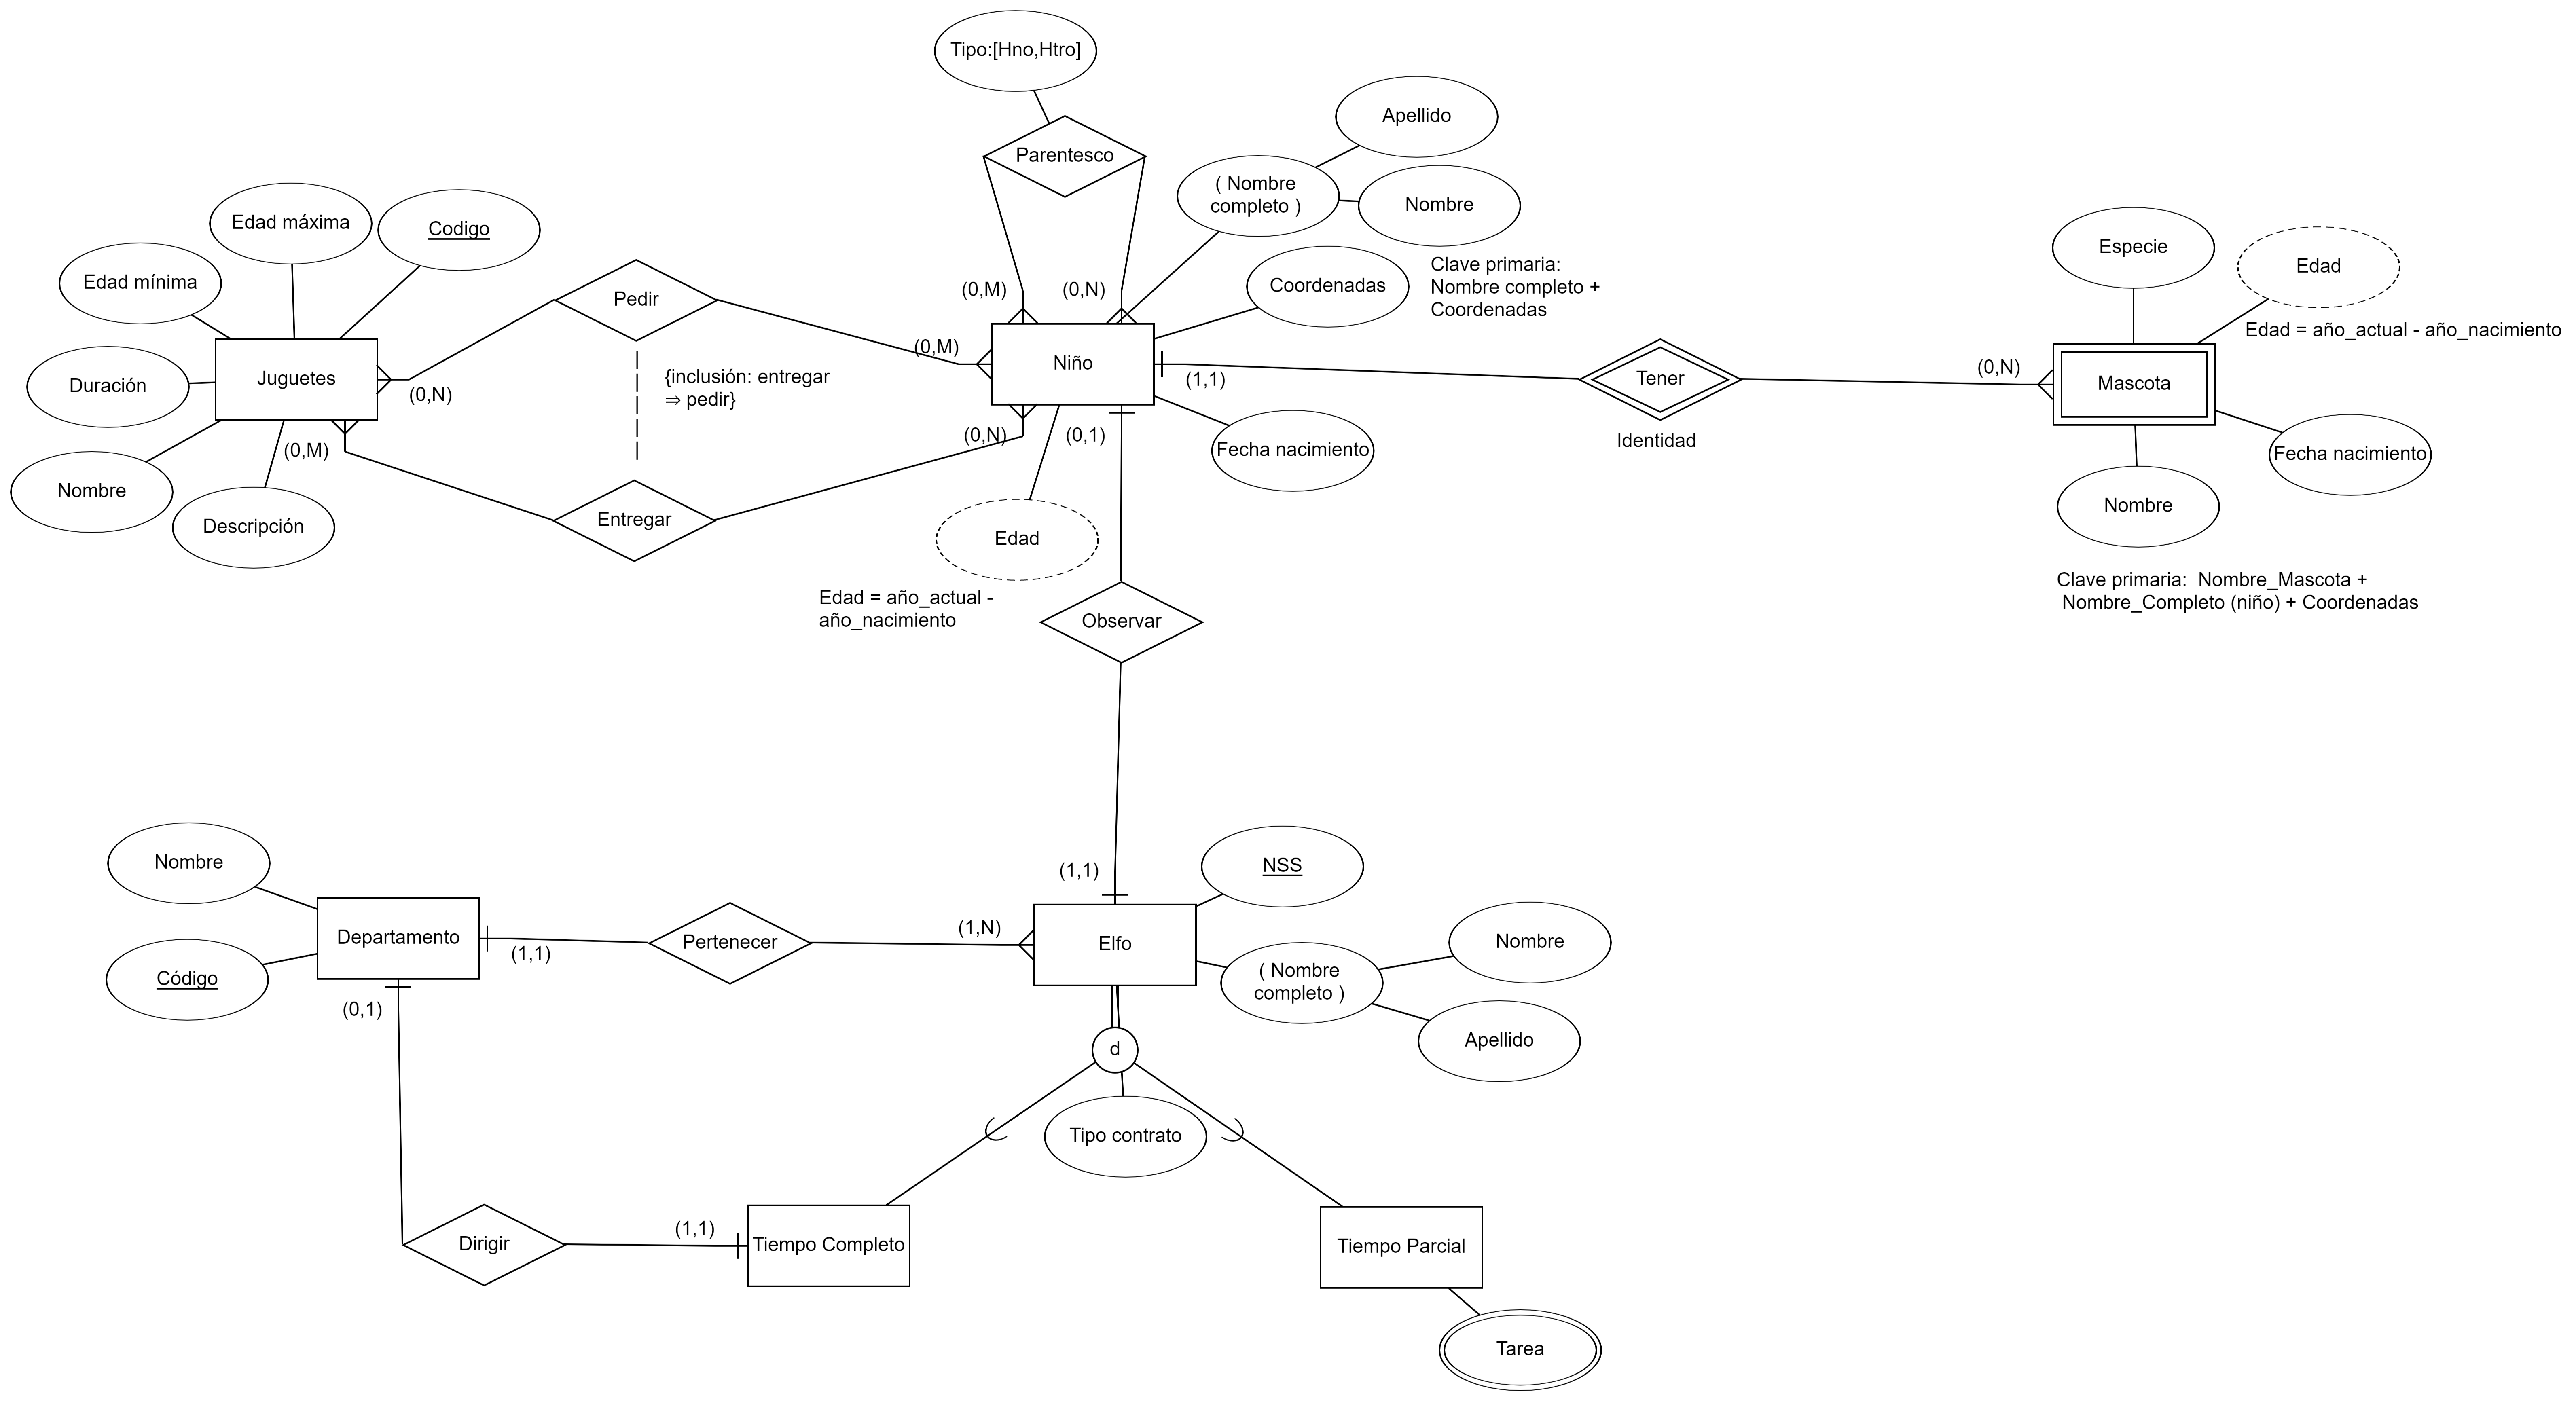
\includegraphics[scale = 0.15, angle = 90]{Modelo/Arthur Christmas ER}
\end{figure}

\newpage 

\begin{hipad}.\\
	\begin{itemize}
		\item Se considera niño a todo menor de 18 años.
		\item Se asume que hay más elfos que niños. Por tanto, puede haber elfos que no observen niños. 
	\end{itemize}
\end{hipad}
	
\begin{noinc}.\\
	\begin{itemize}
		\item Inclusión. Para que un juguete sea entregado a un niño, este debe haberlo pedido previamente. 
		\item El juguete debe ser apto para la edad del niño:
			$$
				Edad\_min \leq Edad\_ni\text{\emph{ñ}}o \leq Edad\_max
			$$
		\item Una persona deja de considerarse un niño el año que cumple la mayoría de edad.
		$$
			Edad < 18\ a\text{\emph{ñ}}os
		$$
	\end{itemize}
\end{noinc}

\newpage

\part*{Modelo relacional}

	\begin{tikzpicture}[relation/.style={rectangle split, rectangle split parts=#1, rectangle split part align=base, draw, anchor=center, align=center, text height=3mm, text centered}]\hspace*{-0.3cm}
	
		% RELATIONS
		
		\node (elfotitle) {\textbf{ELFOS}};
		
		\node [relation=5, rectangle split horizontal, rectangle split part fill={lightgray!50}, anchor=north west, below=0.6cm of elfotitle.west, anchor=west] (elfos)
		{\underline{NSS\_elfo}%
		\nodepart{two}   nombre\_elfo
		\nodepart{three} apellido\_elfo
		\nodepart{four} tipo\_contrato
		\nodepart{five} ID\_departamento};
		
		\node [below=1.3cm of elfos.west, anchor=west] (parcialtitle) {\textbf{PARCIAL}};
		
		\node [relation=1, rectangle split horizontal, rectangle split part fill={lightgray!50}, below=0.6cm of parcialtitle.west, anchor=west] (parcial)
		{\underline{NSS\_elfo}%
		};
		
		\node [below=1.1cm of parcial.west, anchor=west] (tareastitle) {\textbf{TAREAS}};
		
		\node [relation=2, rectangle split horizontal, rectangle split part fill={lightgray!50}, anchor=north west, below=0.6cm of tareastitle.west, anchor=west] (tareas)
		{\underline{NSS\_elfo}%
		\nodepart{two} \underline{nombre\_tarea}
		};
		
		\node [below=1.4cm of tareas.west, anchor=west] (completotitle) {\textbf{COMPLETO}};
		
		\node [relation=1, rectangle split horizontal, rectangle split part fill={lightgray!50}, anchor=north west, below=0.6cm of completotitle.west, anchor=west] (completo)
		{\underline{NSS\_elfo}%
		};
		
		\node [below=1.3cm of completo.west, anchor=west] (departamentotitle) {\textbf{DEPARTAMENTO}};
		
		\node [relation=3, rectangle split horizontal, rectangle split part fill={lightgray!50}, anchor=north west, below=0.6cm of departamentotitle.west, anchor=west] (departamento)
		{\underline{ID\_departamento}%
		\nodepart{two}   \underline{nombre\_departamento}
		\nodepart{three} \underline{NSS\_director}};
		
		\node [below=1.0cm of departamento.west, anchor=west] (niñostitle) {\textbf{NIÑOS}};
		
		\node [relation=5, rectangle split horizontal, rectangle split part fill={lightgray!50}, anchor=north west, below=0.6cm of niñostitle.west, anchor=west] (niños)
		{\underline{nombre\_niño}%
		\nodepart{two}   \underline{apellido\_niño}
		\nodepart{three} \underline{coordenadas\_niño}
		\nodepart {four} fecha\_nacimiento
		\nodepart {five} NSS\_elfo};
		
		\node [below=1.3cm of niños.west, anchor=west] (parentescotitle) {\textbf{PARENTESCO}};
		
		\node [relation=3, rectangle split horizontal, rectangle split part fill={lightgray!50}, anchor=north west, below=0.6cm of parentescotitle.west, anchor=west] (parentesco)
		{\underline{FK\_niño1}%
		\nodepart{two} \underline{FK\_niño2}
		\nodepart{three} tipo\_hermandad};
		
		\node [below=1.3cm of parentesco.west, anchor=west] (mascotastitle) {\textbf{MASCOTAS}};
		
		\node [relation=4, rectangle split horizontal, rectangle split part fill={lightgray!50}, anchor=north west, below=0.6cm of mascotastitle.west, anchor=west] (mascotas)
		{\underline{FK\_niño}%
		\nodepart{two} \underline{nombre\_mascota}
		\nodepart{three} especie
		\nodepart{four} fecha\_nacimiento\_mascota};
		
		\node [below=1.3cm of mascotas.west, anchor=west] (juguetestitle) {\textbf{JUGUETES}};
		
		\node [relation=6, rectangle split horizontal, rectangle split part fill={lightgray!50}, anchor=north west, below=0.6cm of juguetestitle.west, anchor=west] (juguetes)
		{\underline{EAN}%
		\nodepart{two} nombre\_juguete
		\nodepart{three} descripción
		\nodepart{four} duración
		\nodepart{five} edad\_min
		\nodepart{six} edad\_max};
		
		\node [below=1.3cm of juguetes.west, anchor=west] (pedidostitle) {\textbf{PEDIDOS}};
		
		\node [relation=2, rectangle split horizontal, rectangle split part fill={lightgray!50}, anchor=north west, below=0.6cm of pedidostitle.west, anchor=west] (pedidos)
		{\underline{FK\_niño}%
		\nodepart{two} \underline{EAN}};
		
		\node [below=1.3cm of pedidos.west, anchor=west] (entregadostitle) {\textbf{ENTREGADOS}};
		
		\node [relation=2, rectangle split horizontal, rectangle split part fill={lightgray!50}, anchor=north west, below=0.6cm of entregadostitle.west, anchor=west] (entregados)
		{\underline{FK\_niño}%
		\nodepart{two} \underline{EAN}};
		
		% FOREIGN KEYS
		\draw[-latex] (parcial.one south) -- ++(-0,-0.2) -| ($(parcial.one south) + (2,0)$) |- ($(elfos.one south) + (0.25,-0.65)$) -| ($(elfos.one south) - (0.5,0)$);
		
		\draw[-latex] (tareas.one south) -- ++(-0,-0.2) -| ($(tareas.one south) + (3.8,0)$) |- ($(elfos.one south) + (0.25,-0.58)$) -| ($(elfos.one south) + (-0.38,0)$);
		
		\draw[-latex] (completo.one south) -- ++(-0,-0.2) -| ($(completo.one south) + (4,0)$) |- ($(elfos.one south) + (0.25,-0.50)$) -| ($(elfos.one south) + (-0.26,0)$);
		
		\draw[-latex] (departamento.three south) -- ++(-0,-0.2) -| ($(departamento.three south) + (1.5,0)$) |- ($(elfos.one south) + (0.25,-0.40)$) -| ($(elfos.one south) + (-0.14,0)$);
		
		\draw[-latex] (elfos.five north) -- ++(-0, +0.9) -| ($(elfos.one north) - (2,0)$) |- ($(departamento.one south) + (-2, -0.25)$) -| ($(departamento.one south) + (0.25,0)$);
		
		\draw[-latex] (niños.five south) -- ++(-0,-0.25) -| ($(niños.five south) + (1.5 ,0)$) |- ($(elfos.one south) + (0, -0.5)$) -| ($(elfos.one south) + (0,0)$);
		%
		
		\draw[-latex] (parentesco.one south) -- ++(-0,-0.25) -| ($(parentesco.one south) - (2,0)$) |- ($(niños.one south) + (0, -0.5)$) -| ($(niños.one south) + (0,0)$);
		
		\draw[-latex] (parentesco.one south) -- ++(-0,-0.25) -| ($(parentesco.one south) - (2,0)$) |- ($(niños.two south) + (0, -0.5)$) -| ($(niños.two south) + (0,0)$);
		
		\draw[-latex] (parentesco.one south) -- ++(-0,-0.25) -| ($(parentesco.one south) - (2,0)$) |- ($(niños.three south) + (0, -0.5)$) -| ($(niños.three south) + (0,0)$);
		%
		
		\draw[-latex] (parentesco.two south) -- ++(-0,-0.25) -| ($(parentesco.one south) - (2,0)$) |- ($(niños.one south) + (0, -0.5)$) -| ($(niños.one south) + (0,0)$);
		
		\draw[-latex] (parentesco.two south) -- ++(-0,-0.25) -| ($(parentesco.one south) - (2,0)$) |- ($(niños.two south) + (0, -0.5)$) -| ($(niños.two south) + (0,0)$);
		
		\draw[-latex] (parentesco.two south) -- ++(-0,-0.25) -| ($(parentesco.one south) - (2,0)$) |- ($(niños.three south) + (0, -0.5)$) -| ($(niños.three south) + (0,0)$);
		%
		
		\draw[-latex] (mascotas.one south) -- ++(-0,-0.25) -| ($(parentesco.one south) - (2,0)$) |- ($(niños.one south) + (0, -0.5)$) -| ($(niños.one south) + (0,0)$);
		
		\draw[-latex] (mascotas.one south) -- ++(-0,-0.25) -| ($(parentesco.one south) - (2,0)$) |- ($(niños.two south) + (0, -0.5)$) -| ($(niños.two south) + (0,0)$);
		
		\draw[-latex] (mascotas.one south) -- ++(-0,-0.25) -| ($(parentesco.one south) - (2,0)$) |- ($(niños.three south) + (0, -0.5)$) -| ($(niños.three south) + (0,0)$);
		%
		
		\draw[-latex] (pedidos.one south) -- ++(-0,-0.25) -| ($(parentesco.one south) - (2,0)$) |- ($(niños.one south) + (0, -0.5)$) -| ($(niños.one south) + (0,0)$);
		
		\draw[-latex] (pedidos.one south) -- ++(-0,-0.25) -| ($(parentesco.one south) - (2,0)$) |- ($(niños.two south) + (0, -0.5)$) -| ($(niños.two south) + (0,0)$);
		
		\draw[-latex] (pedidos.one south) -- ++(-0,-0.25) -| ($(parentesco.one south) - (2,0)$) |- ($(niños.three south) + (0, -0.5)$) -| ($(niños.three south) + (0,0)$);
		%
		
		\draw[-latex] (entregados.one south) -- ++(-0,-0.25) -| ($(parentesco.one south) - (2,0)$) |- ($(niños.one south) + (0, -0.5)$) -| ($(niños.one south) + (0,0)$);
		
		\draw[-latex] (entregados.one south) -- ++(-0,-0.25) -| ($(parentesco.one south) - (2,0)$) |- ($(niños.two south) + (0, -0.5)$) -| ($(niños.two south) + (0,0)$);
		
		\draw[-latex] (entregados.one south) -- ++(-0,-0.25) -| ($(parentesco.one south) - (2,0)$) |- ($(niños.three south) + (0, -0.5)$) -| ($(niños.three south) + (0,0)$);
		%
		
		\draw[-latex] (pedidos.two south) -- ++(-0,-0.25) -| ($(pedidos.two south) + (2,0)$) |- ($(juguetes.one south) + (0, -0.5)$) -| ($(juguetes.one south) + (0,0)$);
		%
		
		\draw[-latex] (entregados.two south) -- ++(-0,-0.25) -| ($(pedidos.two south) + (2,0)$) |- ($(juguetes.one south) + (0, -0.5)$) -| ($(juguetes.one south) + (0,0)$);
		

		\begin{comment}
			% FOREIGN KEYS
			\draw[-latex] (parcial.one south) -- ++(-0,-0.2) -| ($(parcial.one south) + (2,0)$) |- ($(elfos.one south) + (0.25,-0.50)$) -| ($(elfos.one south) - (0,0)$);
			
			\draw[-latex] (tareas.one south) -- ++(-0,-0.2) -| ($(tareas.one south) + (4,0)$) |- ($(elfos.one south) + (0.25,-0.50)$) -| ($(elfos.one south) + (0,0)$);
			
			\draw[-latex] (completo.one south) -- ++(-0,-0.2) -| ($(completo.one south) + (4,0)$) |- ($(elfos.one south) + (0.25,-0.50)$) -| ($(elfos.one south) + (0,0)$);
			
			\draw[-latex] (departamento.three south) -- ++(-0,-0.2) -| ($(departamento.three south) + (1.5,0)$) |- ($(elfos.one south) + (0.25,-0.50)$) -| ($(elfos.one south) + (0,0)$);
			
			\draw[-latex] (elfos.five north) -- ++(-0, +0.9) -| ($(elfos.one north) - (2,0)$) |- ($(departamento.one south) + (-2, -0.25)$) -| ($(departamento.one south) + (0.25,0)$);
			
			\draw[-latex] (niños.five south) -- ++(-0,-0.25) -| ($(niños.five south) + (1.5 ,0)$) |- ($(elfos.one south) + (0, -0.5)$) -| ($(elfos.one south) + (0,0)$);
			%
			
			\draw[-latex] (parentesco.one south) -- ++(-0,-0.25) -| ($(parentesco.one south) - (2,0)$) |- ($(niños.one south) + (0, -0.5)$) -| ($(niños.one south) + (0,0)$);
			
			\draw[-latex] (parentesco.one south) -- ++(-0,-0.25) -| ($(parentesco.one south) - (2,0)$) |- ($(niños.two south) + (0, -0.5)$) -| ($(niños.two south) + (0,0)$);
			
			\draw[-latex] (parentesco.one south) -- ++(-0,-0.25) -| ($(parentesco.one south) - (2,0)$) |- ($(niños.three south) + (0, -0.5)$) -| ($(niños.three south) + (0,0)$);
			%
			
			\draw[-latex] (parentesco.two south) -- ++(-0,-0.25) -| ($(parentesco.one south) - (2,0)$) |- ($(niños.one south) + (0, -0.5)$) -| ($(niños.one south) + (0,0)$);
			
			\draw[-latex] (parentesco.two south) -- ++(-0,-0.25) -| ($(parentesco.one south) - (2,0)$) |- ($(niños.two south) + (0, -0.5)$) -| ($(niños.two south) + (0,0)$);
			
			\draw[-latex] (parentesco.two south) -- ++(-0,-0.25) -| ($(parentesco.one south) - (2,0)$) |- ($(niños.three south) + (0, -0.5)$) -| ($(niños.three south) + (0,0)$);
			%
			
			\draw[-latex] (mascotas.one south) -- ++(-0,-0.25) -| ($(parentesco.one south) - (2,0)$) |- ($(niños.one south) + (0, -0.5)$) -| ($(niños.one south) + (0,0)$);
			
			\draw[-latex] (mascotas.one south) -- ++(-0,-0.25) -| ($(parentesco.one south) - (2,0)$) |- ($(niños.two south) + (0, -0.5)$) -| ($(niños.two south) + (0,0)$);
			
			\draw[-latex] (mascotas.one south) -- ++(-0,-0.25) -| ($(parentesco.one south) - (2,0)$) |- ($(niños.three south) + (0, -0.5)$) -| ($(niños.three south) + (0,0)$);
			%
			
			\draw[-latex] (pedidos.one south) -- ++(-0,-0.25) -| ($(parentesco.one south) - (2,0)$) |- ($(niños.one south) + (0, -0.5)$) -| ($(niños.one south) + (0,0)$);
			
			\draw[-latex] (pedidos.one south) -- ++(-0,-0.25) -| ($(parentesco.one south) - (2,0)$) |- ($(niños.two south) + (0, -0.5)$) -| ($(niños.two south) + (0,0)$);
			
			\draw[-latex] (pedidos.one south) -- ++(-0,-0.25) -| ($(parentesco.one south) - (2,0)$) |- ($(niños.three south) + (0, -0.5)$) -| ($(niños.three south) + (0,0)$);
			%
			
			\draw[-latex] (entregados.one south) -- ++(-0,-0.25) -| ($(parentesco.one south) - (2,0)$) |- ($(niños.one south) + (0, -0.5)$) -| ($(niños.one south) + (0,0)$);
			
			\draw[-latex] (entregados.one south) -- ++(-0,-0.25) -| ($(parentesco.one south) - (2,0)$) |- ($(niños.two south) + (0, -0.5)$) -| ($(niños.two south) + (0,0)$);
			
			\draw[-latex] (entregados.one south) -- ++(-0,-0.25) -| ($(parentesco.one south) - (2,0)$) |- ($(niños.three south) + (0, -0.5)$) -| ($(niños.three south) + (0,0)$);
			%
			
			\draw[-latex] (pedidos.two south) -- ++(-0,-0.25) -| ($(pedidos.two south) + (2,0)$) |- ($(juguetes.one south) + (0, -0.5)$) -| ($(juguetes.one south) + (0,0)$);
			%
			
			\draw[-latex] (entregados.two south) -- ++(-0,-0.25) -| ($(pedidos.two south) + (2,0)$) |- ($(juguetes.one south) + (0, -0.5)$) -| ($(juguetes.one south) + (0,0)$);
		\end{comment}

	\end{tikzpicture}


\end{document}